\chapter{Improvements}
We could improve our results by both managing our team work more efficiently and also by coding the program in a way that is both faster and more accurate.
\section{Vices in teamwork}
We had a bit of a bumpy start in this project wich would cause some troubles later on.

For starters we had some problems putting together the group. This caused some delay at first, but luckily Kenneth and Erisa could join Group 4. Although we were more team members we had some trouble having a shared understanding of the code as the group was already on their way. This caused  a split in the group that led to 2 members sharing the responsibility for the coding part while the others dealt with thoery and documentation. This seemed to work for a while, but after easter Marius and Gjøran went to USA for an excursion and Kenneth was absent due to illness. This set our development way back and would probably be why we did not finish our implementation of the program as planned. This should have been coordinated and arranged for, but wasn't. Making everyone more included in all aspects of the project, so that missing some team members would not have such an impact, would also decrease the risk of not being able to finish.

\section{Vices in coding}
Although we did not finish we are able to see ways of improving our architecture and design. One way is to get feedback from the user. One idea consists of selecting important terms from the documents that have been identified as relevant by the user, and enchancing the importance of these terms in a new query formulation \cite{MIR}.

Also we could do more document preprocessing like lexical analysis and index term selection. This action should be done by a specialist and implied more time to implement. Furthermore, we could expand the queries with relevant words by construction of term categorization structures like thesaurus.

Further classical vector space models such as VSM and term weighting schemes such as TF and TF-IDF were not initially designed to support different formats of text documents we could use a Semantic-Sensitive Web Information Retrieval Model for HTML Documents that consists of a vector model called Semantic-Sensitive Web Vector Model (SWVM) and a term weighting scheme called Boosted Term Frequency-Inverse Document Frequency (BTF-IDF) in order to retrieve documents from handbook \cite{SSWI}.

\section{Vices in architecture}
We started out by writing our code kind of in parallell with the assignment. After a while we saw the need for an overview of our program. This is something should have thought of before we started coding and might be one of the reasons that our code became somewhat unstructured and hard to work with. Later on we came across an architecture that would greatly help us organize our project and code \cite{MIR}.

\begin{figure}[h]
\centering
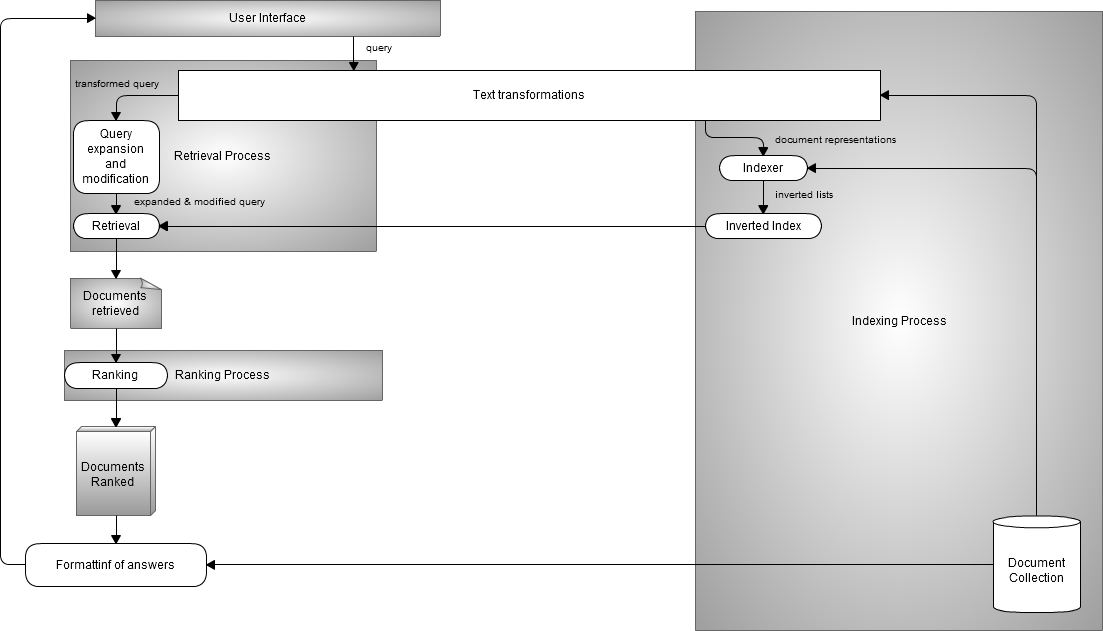
\includegraphics[scale=0.33]{improvements/alternative_architecture.png}
\caption{Proposal of architecture}
\end{figure}